\chapter{QED: Quantum Field Interaction Theory Applied to EM}
\section{Dyson-Wick's Expansion/or QED Hamiltonian Density}
The Dyson expansion of the S operator is
\begin{equation}
S=I-i \int_{-\infty}^{\infty} \mathcal{H}_{I}^{I}\left(x_{1}\right) d^{4} x_{1}-\frac{1}{2 !} \int_{-\infty}^{\infty} T\left\{\mathcal{H}_{I}^{I}\left(x_{1}\right) \mathcal{H}_{l}^{I}\left(x_{2}\right)\right\} d^{4} x_{1} d^{4} x_{2}+\ldots .
\label{dyson-wick-expansion}
\end{equation}
For the interaction Hamiltonian density in (\ref{dyson-wick-expansion}) we use the relation discovered to work for RQM, because we have learned that Hamiltonians for RQM expressed in the Schrödinger Picture, as a rule, take the same form for QFT expressed in the Heisenberg Picture. We are working in the Interaction Picture, for which operators (such as the Hamiltonian density) take the same form in the I.P. as in the H.P. So, for electromagnetic interactions between electrons, positrons, and photons, the quantum Hamiltonian density takes the form, where, $A_{\mu}\gamma^{\mu}=\cancel{A}$
\begin{equation}
\mathcal{H}_{I}^{I}=-\mathcal{L}_{I}^{I}=-e \bar{\psi} A_{\mu} \gamma^{\mu} \psi=-e \bar{\psi} \cancel{A} \psi=-e\left(\bar{\psi}^{+}+\bar{\psi}^{-}\right)\left(A^{+}+\bar{A}^{-}\right)\left(\psi^{+}+\psi^{-}\right)
\end{equation}
and
\begin{equation}
S=\underbrace{I}_{S^{(0)}} + \underbrace{i e \int_{-\infty}^{\infty}(\bar{\psi} \cancel{A} \psi)_{x_{1}} d^{4} x_{1}}_{S^{(1)}}-\underbrace{\frac{1}{2 !} e^{2} \int_{-\infty}^{\infty} \int_{-\infty}^{\infty} T\left\{(\bar{\psi} \cancel{A} \psi)_{x_{1}}(\bar{\psi} \cancel{A} \psi)_{x_{2}}\right\} d^{4} x_{1} d^{4} x_{2}}_{S^{(2)}}+\dots
\label{explicit-S}
\end{equation}
\bluep{We can approximate (\ref{explicit-S}) by taking only the first few terms.} In this chapter, we only deal with $S^{(0)},S^{(1)},S^{(2)}$.

The second term in (\ref{explicit-S}) has factors operating all at the same time $t_1$, and so can be considered time ordered. Wick's theorem for this case reduces to
$$T\left\{(A B \ldots)_{x_{1}}\right\}=N\left\{(A B \ldots)_{x_{1}}\right\}$$
$$
S^{(1)}=i e \int_{-\infty}^{\infty} N\{\bar{\psi} \cancel{A} \psi\}_{x_{1}} d^{4} x_{1}
$$
\section{Physical Meaning of S(1)}
Consider $S^{(1)}$ term on an initial state
\begin{equation}
S^{(1)}|i\rangle=(-i) \int d^{4} x_{1} N\{-e \bar{\psi} \cancel{A} \psi\}_{x_{1}}|i\rangle= i \int d^{4} x_{1} N\left\{e\left(\bar{\psi}^{+}+\bar{\psi}\right)\left(\cancel{A}^{+}+\cancel{A}^{-}\right)\left(\psi^{+}+\psi^{-}\right)\right\}_{x_{1}}|i\rangle
\label{S(1)}
\end{equation}
If we multiply out the factors in (\ref{S(1)}) we will have eight different sub-terms contributing to the
$S^{(1)}$ term in $S .$ We will label these sub-terms as $S_{j}^{(1)}$ where $j=1,2, \ldots, 8$. For example
$$
\left.S_{1}^{(1)} | e_{p_{1}, q}^{-}, e_{p_{2}, r_{2}}^{+}\right\rangle=i e \int d^{4} x_{1} N\left\{\bar{\psi}^{+} A^-_{\mu} \gamma^{\mu} \psi^{+}\right\}_{x_{1}}\left|e_{p_{1}, r_{1}}^{-}, e_{p_{2}, r_{2}}^{+}\right\rangle\left.=i e \int d^{4} x_{1}\left\{A_{\mu}^{-} \bar{\psi}^{+} \gamma^{\mu} \psi^{+}\right\}_{x_{1}} | e_{\mathrm{p}_{1}, r_{1}}^{-}, e_{p_{2}, r_{2}}^{+}\right\rangle
$$
Substituting the expressions for the photon and spinor fields, we have
$$
S_{1}^{(1)}\left|e_{p_{1}, n}^{-}, e_{p_{2}, r_{2}}^{+}\right\rangle= i e \int d^{4} x_{1}\left(\sum_{s, k} \sqrt{\frac{1}{2 V{\omega_{k}}}} \varepsilon_{\mu, s}(\mathbf{k}) a_{s}^{\dagger}(\mathbf{k}) e^{i kx_1}\right)\left(\sum_{r^{\prime}, p^{\prime}} \sqrt{\frac{m}{V E_{p^{\prime}}}} d r^{\prime}\left(p^{\prime}\right) \bar{v}_{r^{\prime}}\left(p^{\prime}\right) e^{-i p^{\prime} x_{1}}\right) \gamma^{\mu}\times
$$
$$
\left(\sum_{r^{''}, p^{''}} \sqrt{\frac{m}{V E_{p^{''}}}} c_{r^{''}}\left(p^{\prime \prime}\right) u_{r^{''}}\left(p^{''e}\right) e^{-p^{''} \gamma_{1}^{''}}\right)\left.| e_{p_{1}, r_{2}}^{-}, e^{+}_{ p_{2}, r_{2}}\right\rangle
$$
Destruction operators $d_{r^{\prime}}$ and $c_{r^{\prime \prime}}$ will destroy the ket (i.e., make it equal to zero) for all terms in the sum except when i) $p^{\prime}=p_{2}$ and $r^{\prime}=r_{2},$ and when in $r^{\prime \prime}=r_{1}$. Those will reduce the ket to the vacuum state by destroying the electron and positron we started out with. Thus, we have 
$$
\left.S_{1}^{(1)} | e_{p_{1}, r_{1}}^{-}, e_{p_{2}, r_{2}}^{+}\right\rangle=
$$
$$
ie  \int d^{4} x_{1}\left\{\left(\sum_{s, k} \sqrt{\frac{1}{2 V{\omega_{k}}}} \varepsilon_{\mu, s}(\mathbf{k}) a_{s}^{\dagger}(\mathbf{k}) e^{i kx_1}\right)\right.\left.\frac{m}{V} \sqrt{\frac{1}{E_{p_{1}} E_{p 2}}} \bar{v}_{r_{2}}\left(p_{2}\right) e^{-i p_{2} x_{1}} \gamma^{\mu} u_{r_1}\left(p_{1}\right) e^{-i p_{1} x_{1}}\right\}|0\rangle
$$
Each term of the remaining sum above creates a photon with different momentum and polarization states. So
$$
\left.S_{1}^{(1)} | e_{\mathrm{p}_{1}, r_{1}}^{-}, e_{\mathrm{p}_{2}, r_{2}}^{+}\right)=
$$
$$
ie \int d^{4} x_{1}\left\{\sum_{s, k} \sqrt{\frac{1}{2 V\omega_k}} \varepsilon_{\mu, s}(\mathbf{k}) e^{i kx_1} \frac{m}{V} \sqrt{\frac{1}{E_{p_1} E_{p_{2}}}} \bar{v}_{r_{2}}\left(\mathbf{p}_{2}\right) e^{-i p_{2} x_{1}} \gamma^{\mu} u_{r_1}\left(\mathbf{p}_{1}\right) e^{-i p_{1} x_{1}}\right\}\left|\gamma_{\mathbf{k}, s}\right\rangle
$$
Suppose $\left|\gamma_{\mathbf{k}_1, s_1}\right\rangle$ is our final state of a single photon. For this final state, note that
$$
\left\langle\gamma_{\mathbf{k}_{1},s_{1}}\left|S_{1}^{(1)}\right| e_{\mathbf{p}_{1}, r_{1}}^{-}, e_{\mathrm{p}_{2}, r_{2}}^{+}\right\rangle=S_{1, f i}^{(1)}
$$
which is the transition amplitude for the following Feynman diagram
\begin{figure}[H]
    \centering
    
\tikzset{every picture/.style={line width=0.75pt}} %set default line width to 0.75pt        

\begin{tikzpicture}[x=0.75pt,y=0.75pt,yscale=-1,xscale=1]
%uncomment if require: \path (0,300); %set diagram left start at 0, and has height of 300

%Straight Lines [id:da307650809518932] 
\draw    (58,58.37) -- (158,158.37) ;
%Straight Lines [id:da4053696323117585] 
\draw    (158,158.37) -- (59.87,247.8) ;
%Shape: Wave [id:dp5998613246245391] 
\draw   (157,157.8) .. controls (161.14,161.39) and (165.11,164.8) .. (169.63,164.8) .. controls (174.16,164.8) and (177.99,161.39) .. (182,157.8) .. controls (186.01,154.21) and (189.84,150.8) .. (194.37,150.8) .. controls (198.89,150.8) and (202.85,154.21) .. (207,157.8) .. controls (211.14,161.39) and (215.11,164.8) .. (219.63,164.8) .. controls (224.16,164.8) and (227.99,161.39) .. (232,157.8) .. controls (236.01,154.21) and (239.84,150.8) .. (244.37,150.8) .. controls (248.89,150.8) and (252.85,154.21) .. (257,157.8) .. controls (261.14,161.39) and (265.11,164.8) .. (269.63,164.8) .. controls (274.16,164.8) and (277.99,161.39) .. (282,157.8) .. controls (286.01,154.21) and (289.84,150.8) .. (294.37,150.8) .. controls (298.89,150.8) and (302.85,154.21) .. (307,157.8) .. controls (311.14,161.39) and (315.11,164.8) .. (319.63,164.8) .. controls (324.16,164.8) and (327.99,161.39) .. (332,157.8) .. controls (332,157.8) and (332,157.8) .. (332,157.8) ;
%Shape: Triangle [id:dp4766081790625024] 
\draw  [fill={rgb, 255:red, 0; green, 0; blue, 0 }  ,fill opacity=1 ] (115.33,115.49) -- (97.69,104.32) -- (103.66,98.17) -- cycle ;
%Shape: Triangle [id:dp2439506934283957] 
\draw  [fill={rgb, 255:red, 0; green, 0; blue, 0 }  ,fill opacity=1 ] (101.73,210.33) -- (113.1,192.82) -- (119.17,198.86) -- cycle ;

% Text Node
\draw (86,61.37) node    {$e^{-}$};
% Text Node
\draw (88,244.37) node    {$e^{+}$};
% Text Node
\draw (162,183.37) node    {$x_{1}$};
% Text Node
\draw (326,138.37) node    {$\gamma $};


\end{tikzpicture}

    \caption{Single vertex interaction}
    \label{fig:single-vertex}
\end{figure}
From equations above, where all terms having different bra and ket states drop out,
$$
S_{1, f i}^{(1)}=i e \int d^{4} x_{1}\left\{\sqrt{\frac{1}{2 V \omega_{k_{1}}}} \varepsilon_{\mu, s_{1}}\left(\mathbf{k}_{1}\right) e^{i k_{1} x_{1}} \frac{m}{V}\right.\left.\sqrt{\frac{1}{E_{p_{1}} E_{p_{2}}}} \bar{v}_{r_{2}}\left(\mathbf{p}_{2}\right) e^{-i p_{2} x_{1}} \gamma^{\mu} u_{r_{1}}\left(\mathbf{p}_{1}\right) e^{-i p_{1} x_{1}}\right\}\left\langle\gamma \| \gamma\right\rangle
$$
$$
=ie \frac{m}{\sqrt{2 V^{3}}} \sqrt{\frac{1}{\omega_{\mathrm{k}_{1}} E_{\mathrm{p}_{1}} E_{\mathrm{p}_{2}}}} \varepsilon_{\mu, s_{1}}\left(\mathrm{k}_{1}\right) \bar{v}_{\mathrm{r}_{2}}\left(\mathrm{p}_{2}\right) \gamma^{\mu} u_{r_1}\left(\mathrm{p}_{1}\right)\underbrace{\int e^{i\left(k_{1}-p_{2}-p_{1}\right) x_{1}} d^{4} x_{1}}_{(2 \pi)^{4} \delta^{(4)}\left(k_{1}-p_{2}-p_{1}\right)}
$$
\begin{equation}
    =i e(2 \pi)^{4} \delta^{(4)}\left(k_{1}-p_{2}-p_{1}\right) \sqrt{\frac{1}{2 V \omega_{1}}} \sqrt{\frac{m}{V_{\mathrm{p}}}} \sqrt{\frac{m}{V E_{p_{2}}}} \varepsilon_{\mu, s_{1}}\left(\mathbf{k}_{1}\right) \bar{v}_{r_{2}}\left(\mathbf{p}_{2}\right) \gamma^{\mu} u_{\mathrm{r_1}}\left(\mathbf{p}_{1}\right)
    \label{S-1-fi}
\end{equation}
The Dirac delta function arising
in our calculation ensures that \redp{the outgoing 4-momentum of the final state photon equals the incoming total 4-momentum of the two initial state particles.} This, we will see, is a general principle that holds for all transition amplitudes, throughout QFT. Outgoing 4-momentum for any interaction vertex (three particles interacting at a
point in a Feynman diagram) equals incoming 4-momentum.

\textbf{\redp{The interaction represented mathematically above and pictorially by Fig. (\ref{fig:single-vertex}) is not physically viable and does not occur.}}
\begin{center}
\tikzset{every picture/.style={line width=0.75pt}} %set default line width to 0.75pt        

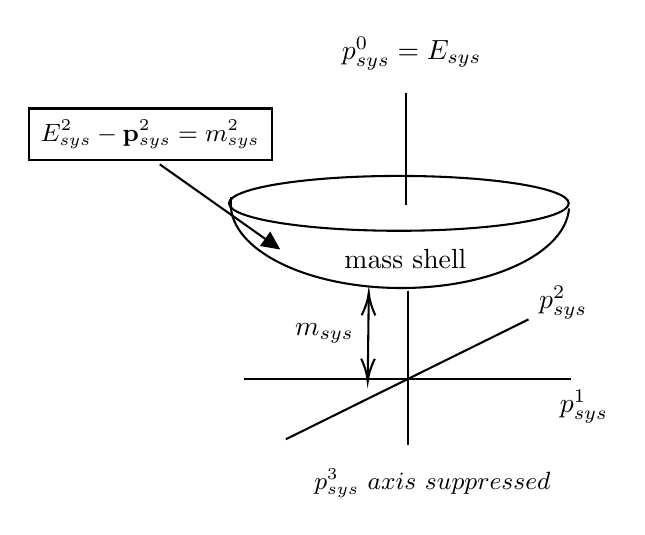
\begin{tikzpicture}[x=0.75pt,y=0.75pt,yscale=-1,xscale=1]
%uncomment if require: \path (0,300); %set diagram left start at 0, and has height of 300

%Shape: Ellipse [id:dp5571456664169634] 
\draw   (405,104.58) .. controls (405,97.28) and (441.64,91.37) .. (486.83,91.37) .. controls (532.03,91.37) and (568.67,97.28) .. (568.67,104.58) .. controls (568.67,111.88) and (532.03,117.8) .. (486.83,117.8) .. controls (441.64,117.8) and (405,111.88) .. (405,104.58) -- cycle ;
%Shape: Arc [id:dp5755134037737296] 
\draw  [draw opacity=0] (568.82,107.06) .. controls (567.12,128.58) and (531.16,145.6) .. (487.13,145.37) .. controls (442.1,145.14) and (405.69,126.94) .. (405.81,104.73) .. controls (405.81,103.68) and (405.9,102.64) .. (406.06,101.61) -- (487.34,105.16) -- cycle ; \draw   (568.82,107.06) .. controls (567.12,128.58) and (531.16,145.6) .. (487.13,145.37) .. controls (442.1,145.14) and (405.69,126.94) .. (405.81,104.73) .. controls (405.81,103.68) and (405.9,102.64) .. (406.06,101.61) ;
%Straight Lines [id:da112253833250195] 
\draw    (490.34,51.59) -- (490.34,105.16) ;
%Straight Lines [id:da11852275241679622] 
\draw    (491.34,146.59) -- (491.34,220.8) ;
%Straight Lines [id:da8670761805887259] 
\draw    (412,189.37) -- (569.67,189.37) ;
%Straight Lines [id:da3801545380094623] 
\draw    (432.38,218.24) -- (549.29,160.5) ;
%Straight Lines [id:da8071395461508041] 
\draw    (471.86,188.37) -- (472.32,149.59) ;
\draw [shift={(472.34,147.59)}, rotate = 450.68] [color={rgb, 255:red, 0; green, 0; blue, 0 }  ][line width=0.75]    (10.93,-3.29) .. controls (6.95,-1.4) and (3.31,-0.3) .. (0,0) .. controls (3.31,0.3) and (6.95,1.4) .. (10.93,3.29)   ;
\draw [shift={(471.83,190.37)}, rotate = 270.68] [color={rgb, 255:red, 0; green, 0; blue, 0 }  ][line width=0.75]    (10.93,-3.29) .. controls (6.95,-1.4) and (3.31,-0.3) .. (0,0) .. controls (3.31,0.3) and (6.95,1.4) .. (10.93,3.29)   ;
%Straight Lines [id:da37867462769054516] 
\draw    (371.67,85.8) -- (427.22,125.07) ;
\draw [shift={(429.67,126.8)}, rotate = 215.26] [fill={rgb, 255:red, 0; green, 0; blue, 0 }  ][line width=0.08]  [draw opacity=0] (8.93,-4.29) -- (0,0) -- (8.93,4.29) -- cycle    ;

% Text Node
\draw (451,167.37) node    {$m_{sys}$};
% Text Node
\draw (490,131.37) node   [align=left] {mass shell};
% Text Node
\draw (576,202.37) node    {$p^{1}_{sys}$};
% Text Node
\draw (566,152.37) node    {$p^{2}_{sys}$};
% Text Node
\draw (493,32.37) node    {$p^{0}_{sys} =E_{sys}$};
% Text Node
\draw    (308.5,58.87) -- (425.5,58.87) -- (425.5,83.87) -- (308.5,83.87) -- cycle  ;
\draw (367,71.37) node  [font=\small]  {$E^{2}_{sys} -\mathbf{p}^{2}_{sys} =m^{2}_{sys}$};
% Text Node
\draw (503,239.37) node  [font=\small]  {$p^{3}_{sys} \ axis\ suppressed$};


\end{tikzpicture}

\end{center}
The schematic above shows the following relation:(i.e. a shell upon which real particle energies and 3-momenta values must lie.)
\begin{equation}
E_{s y s}^{2}-\mathbf{p}_{s y s}^{2}=m_{s y s}^{2}
\end{equation}
For a system of particles, we determine an invariant mass $m_{sys}$. The surface in the figure is called the \textbf{mass shell}. Real particles must be "on the mass shell". Virtual particles can be, and generally are "off shell". $m_{sys}=0$ for photons, so the photon mass shell touches the origin.

From the delta function in (\ref{S-1-fi}), we know that the outgoing 4-momentum for the photon of Fig(\ref{fig:single-vertex}) equals the incoming total 4-momentum of the electron and positron:
$$
p_{i}^{\mu}=\left(\begin{array}{l}
{E_{1}+E_{2}} \\
{\mathbf{p}_{1}+\mathbf{p}_{2}}
\end{array}\right)=p_{f}^{\mu}=\left(\begin{array}{c}
{\omega_{k_{1}}} \\
{\mathbf{k}_{1}}
\end{array}\right)
$$
For initial state
$$
p_{i}^{\mu} p_{i \mu}=\left(E_{1}+E_{2}\right)^{2}-\left(\mathbf{p}_{1}+\mathbf{p}_{2}\right) \cdot\left(\mathbf{p}_{1}+\mathbf{p}_{2}\right)=m_{s y s}^{2} \neq 0
$$
For final state
$$
p_{f}^{\mu} p_{f \mu}=\underbrace{\left(E_{1}+E_{2}\right)^{2}}_{\omega_{\mathrm{k}_{1}}}-\underbrace{\left(\mathrm{p}_{1}+\mathrm{p}_{2}\right)}_{\mathrm{k}_{1}} \cdot \underbrace{\left(\mathrm{p}_{1}+\mathrm{p}_{2}\right)}_{\mathrm{k}_{1}}=m_{\mathrm{sys}}^{2} \neq 0
$$
\textbf{which must equal zero for a photon. That it doesn't equal zero means we can't produce a real photon.}
\begin{qt}
    $$
S_{f i}=\left\langle\gamma\left|S_{1}^{(1)} +\underbrace{S_{2}^{(1)}+\ldots+S_{8}^{(1)}}_{\text {all yield zero }}\right| e_{\mathbf{p}_{1}, n}^{-}, e_{\mathbf{p}_{2}, r_{2}}^{+}\right\rangle=\underbrace{\langle\gamma|}_{\text {on-shell }} \underbrace{\left.S_{1}^{(1)} | e_{p_{1}, n}^{-}, e^{+}_{\mathrm{p}_{2}, r_{2}}\right\rangle}_{\text {off-shell photon }}=0
$$
because the only ket left is an off-shell photon with $k^{\mu}=p_{1}^{\mu}+p_{2}^{\mu},$ and that is a different state from, and thus orthogonal to, any real final state photon, which cannot have this value for $k^{\mu} .$ Thus, the transition amplitude for Fig. (\ref{fig:single-vertex}) is zero. Similar logic for all single vertex interactions means we can simply ignore $S^{(1)}$ from here on.
\end{qt}
\section{Physical Meaning of S(2)}
\textbf{$S^{(2)}$ will represent two vertex interactions.} The first term of $S^{(2)}$ is $S_A^{(2)}$:
$$
S_{A}^{(2)}=-\frac{1}{2 !} e^{2} \iint d^{4} x_{1} d^{4} x_{2} N\left\{(\bar{\psi} \cancel{A} \psi)_{x_{1}}(\bar{\psi} \cancel{A} \psi)_{x_{2}}\right\}
$$
\textbf{\redp{This represents two independent processes like $S^{(1)}$.}} The two processes
do not interact with one another and each behaves as if the other did not exist. There is no virtual particle (Feynman propagator) linking them. Think of two separate single vertex Feynman diagrams. Neither of these can occur, so $S_A^{(2)}$ does not represent a real physical process and is ignored in QFT.

\subsection{The photon propagator term}
Consider the second term of $S^{(2)}$ acting on an initial state
\begin{equation}
S_{B}^{(2)}|i\rangle=-\frac{1}{2 !} e^{2} \iint d^{4} x_{1} d^{4} x_{2} N\left\{(\bar{\psi} \linktwoterms{\cancel{A}}{\psi)_{x_{1}}(\bar{\psi}}{\cancel{A}} \psi)_{x_{2}}\right\}|i\rangle
\label{four-external-lepton-interactions}
\end{equation}
The only initial states (\ref{four-external-lepton-interactions}) could destroy would be electron/positron states; and the only final states it could create would be electron/positron states. \textbf{We call these types of interactions four external lepton interactions.}
\begin{figure}[H]
    \centering
\tikzset{every picture/.style={line width=0.75pt}} %set default line width to 0.75pt        
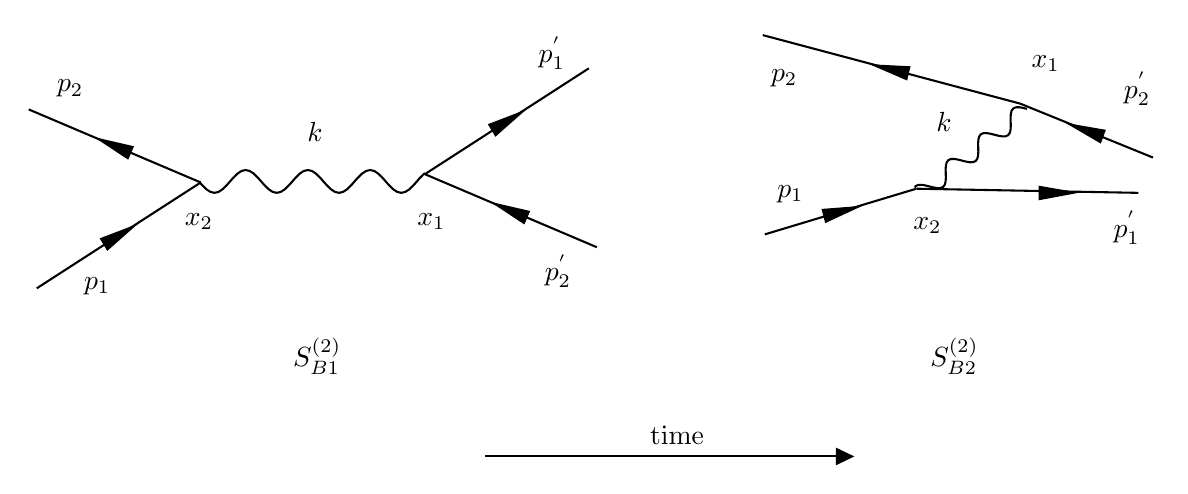
\begin{tikzpicture}[x=0.75pt,y=0.75pt,yscale=-1,xscale=1]
%uncomment if require: \path (0,300); %set diagram left start at 0, and has height of 300

%Straight Lines [id:da29515338597014595] 
\draw    (39,63) -- (121.87,98.2) ;
%Straight Lines [id:da8356384809428652] 
\draw    (121.87,98.2) -- (42.87,149.2) ;
%Shape: Wave [id:dp48547110897765466] 
\draw   (121,97.7) .. controls (123.45,100.52) and (125.79,103.2) .. (128.5,103.2) .. controls (131.21,103.2) and (133.55,100.52) .. (136,97.7) .. controls (138.45,94.88) and (140.79,92.2) .. (143.5,92.2) .. controls (146.21,92.2) and (148.55,94.88) .. (151,97.7) .. controls (153.45,100.52) and (155.79,103.2) .. (158.5,103.2) .. controls (161.21,103.2) and (163.55,100.52) .. (166,97.7) .. controls (168.45,94.88) and (170.79,92.2) .. (173.5,92.2) .. controls (176.21,92.2) and (178.55,94.88) .. (181,97.7) .. controls (183.45,100.52) and (185.79,103.2) .. (188.5,103.2) .. controls (191.21,103.2) and (193.55,100.52) .. (196,97.7) .. controls (198.45,94.88) and (200.79,92.2) .. (203.5,92.2) .. controls (206.21,92.2) and (208.55,94.88) .. (211,97.7) .. controls (213.45,100.52) and (215.79,103.2) .. (218.5,103.2) .. controls (221.21,103.2) and (223.55,100.52) .. (226,97.7) .. controls (227.29,96.21) and (228.56,94.75) .. (229.87,93.72) ;
%Straight Lines [id:da12560516877601058] 
\draw    (308.87,43.2) -- (229.87,94.2) ;
%Straight Lines [id:da6163580842382406] 
\draw    (229.87,94.2) -- (312.73,129.4) ;
%Shape: Triangle [id:dp685466344952348] 
\draw  [fill={rgb, 255:red, 0; green, 0; blue, 0 }  ,fill opacity=1 ] (72.99,77.4) -- (89.03,81.1) -- (86.72,86.49) -- cycle ;
%Shape: Triangle [id:dp005741777290943051] 
\draw  [fill={rgb, 255:red, 0; green, 0; blue, 0 }  ,fill opacity=1 ] (263.86,108.6) -- (279.9,112.3) -- (277.58,117.69) -- cycle ;
%Shape: Triangle [id:dp11625025303653935] 
\draw  [fill={rgb, 255:red, 0; green, 0; blue, 0 }  ,fill opacity=1 ] (89.3,119.51) -- (76.95,130.4) -- (73.92,125.38) -- cycle ;
%Shape: Triangle [id:dp30589288901509604] 
\draw  [fill={rgb, 255:red, 0; green, 0; blue, 0 }  ,fill opacity=1 ] (276.3,64.51) -- (263.95,75.4) -- (260.92,70.38) -- cycle ;
%Straight Lines [id:da5797267371251957] 
\draw    (392.67,27.2) -- (516.67,60.2) ;
%Straight Lines [id:da5534129518575254] 
\draw    (516.67,60.2) -- (580.67,86.2) ;
%Straight Lines [id:da13099665104403413] 
\draw    (393.67,123.2) -- (466.67,101.2) ;
%Straight Lines [id:da23142398769308015] 
\draw    (466.67,101.2) -- (573.67,103.2) ;
%Shape: Triangle [id:dp9580604600019759] 
\draw  [fill={rgb, 255:red, 0; green, 0; blue, 0 }  ,fill opacity=1 ] (438,110.15) -- (423.07,117.08) -- (421.59,111.41) -- cycle ;
%Shape: Triangle [id:dp6776790710702215] 
\draw  [fill={rgb, 255:red, 0; green, 0; blue, 0 }  ,fill opacity=1 ] (542.27,103.15) -- (526.08,106.18) -- (526.05,100.32) -- cycle ;
%Shape: Wave [id:dp647042217139919] 
\draw   (519.94,62.74) .. controls (517.3,62.05) and (514.78,61.39) .. (513.37,62.52) .. controls (511.95,63.64) and (512.03,66.24) .. (512.11,68.97) .. controls (512.2,71.7) and (512.28,74.3) .. (510.86,75.42) .. controls (509.45,76.55) and (506.93,75.89) .. (504.29,75.2) .. controls (501.65,74.51) and (499.14,73.85) .. (497.72,74.98) .. controls (496.3,76.1) and (496.38,78.7) .. (496.47,81.43) .. controls (496.55,84.16) and (496.63,86.76) .. (495.22,87.88) .. controls (493.8,89.01) and (491.28,88.35) .. (488.64,87.66) .. controls (486.01,86.96) and (483.49,86.31) .. (482.07,87.43) .. controls (480.66,88.56) and (480.74,91.16) .. (480.82,93.89) .. controls (480.91,96.61) and (480.98,99.21) .. (479.57,100.34) .. controls (478.15,101.47) and (475.64,100.81) .. (473,100.12) .. controls (470.36,99.42) and (467.84,98.77) .. (466.43,99.89) .. controls (466.19,100.08) and (466,100.31) .. (465.84,100.58) ;
%Shape: Triangle [id:dp3657896804062972] 
\draw  [fill={rgb, 255:red, 0; green, 0; blue, 0 }  ,fill opacity=1 ] (446.78,41.87) -- (463.22,42.67) -- (461.89,48.39) -- cycle ;
%Shape: Triangle [id:dp26512090066334226] 
\draw  [fill={rgb, 255:red, 0; green, 0; blue, 0 }  ,fill opacity=1 ] (541.06,70.42) -- (557.28,73.22) -- (555.27,78.73) -- cycle ;
%Straight Lines [id:da8555170327907058] 
\draw    (258.77,230.2) -- (433.77,230.2) ;
\draw [shift={(436.77,230.2)}, rotate = 180] [fill={rgb, 255:red, 0; green, 0; blue, 0 }  ][line width=0.08]  [draw opacity=0] (8.93,-4.29) -- (0,0) -- (8.93,4.29) -- cycle    ;

% Text Node
\draw (59,53) node    {$p_{2}$};
% Text Node
\draw (72,148) node    {$p_{1}$};
% Text Node
\draw (291,36) node    {$p^{'}_{1}$};
% Text Node
\draw (294,141) node    {$p^{'}_{2}$};
% Text Node
\draw (121,117) node    {$x_{2}$};
% Text Node
\draw (233,117) node    {$x_{1}$};
% Text Node
\draw (177,74) node    {$k$};
% Text Node
\draw (529,41) node    {$x_{1}$};
% Text Node
\draw (472,119) node    {$x_{2}$};
% Text Node
\draw (573,53) node    {$p^{'}_{2}$};
% Text Node
\draw (568,120) node    {$p^{'}_{1}$};
% Text Node
\draw (480,69) node    {$k$};
% Text Node
\draw (406,104) node    {$p_{1}$};
% Text Node
\draw (403,48) node    {$p_{2}$};
% Text Node
\draw (178,182) node    {$S^{( 2)}_{B1}$};
% Text Node
\draw (485,182) node    {$S^{( 2)}_{B2}$};
% Text Node
\draw (351.33,220) node   [align=left] {time};


\end{tikzpicture}

    \caption{Bhabha scattering can occur in two ways}
    \label{fig:Bhabha-scattering}
\end{figure}
In Fig.(\ref{fig:Bhabha-scattering}), both scenarios have the same incoming and outgoing particle states, which are all that we can measure. The internal virtual particle interaction is not measurable so there is no way
we can tell which of the two interactions gave us the Bhabha scattering.Bhabha scattering actually entails both types of interaction, \bluep{i) an annihilation of $e^{-}$ with an $e^{+}$ followed by a creation of the same two types of particles,  and ii) one of the incoming particles emitting a virtual photon which is then absorbed by the other particle. i.e., the same incoming momenta and spins for both and the same outgoing momenta and spins for both.}

\subsubsection{First type of Bhabha Scattering}
Consider the first type of Bhabha scattering with the S operator acting on the incoming state,
\begin{equation}
S_{B}^{(2)}\left|e_{\mathrm{p}_{1}, \mathrm{r_1}}^{-}, e_{\mathrm{p}_{2}, \mathrm{r}_{2}}^{+}\right\rangle=-\frac{1}{2 !} e^{2} \iint d^{4} x_{1} d^{4} x_{2} N\left\{(\bar{\psi} \linktwoterms{\cancel{A}}{ \psi)_{x_{1}}(\bar{\psi}}{\cancel{A}}  \psi)_{x_{2}}\right\}\left|e_{\mathrm{p}_1, \mathrm{r}_1}^{-}, e^{+}_{\mathrm{p}_{2}, r_{2}}\right\rangle
\end{equation}
At $x_{2},$ the $\psi^{+}$ part of $\psi_{x_{2}}$ would destroy the ket electron; the $\bar{\psi}^+$ part of $\bar{\psi}_{x_{2}}$ would destroy the ket positron; and we would be left with the vacuum $|0\rangle$. The propagator would then create a virtual photon at $x_{2}$ and propagate it to $x_{1}$ where it would be destroyed. Then, the $\psi^{-}$ part of $\psi_{x_{1}}$ would create a positron at $x_{1} ;$ and the $\bar{\psi}$ part of $\bar{\psi}_{x_{1}}$ would create an electron there.
$$
S_{B 1}^{(2)}=\frac{-e^{2}}{2}\left\langle e^-_{p_{1}^{\prime}, r^{\prime}_1}, e^{+}_{ p_{2^{\prime}} r_{2}^{\prime}}\right|\iint d^{4} x_{1} d^{4} x_{2}\left((\bar{\psi}^{-} \linktwoterms{\cancel{A}}{ \psi^{-})_{x_{1}}(\bar{\psi}^{+}}{\cancel{A}} \psi^{+})_{x_{2}}+\right.
$$
$$
\left.N\left\{(\bar{\psi}^{+} \linktwoterms{\cancel{A}}{ \psi^{+})_{x_{1}}(\bar{\psi}^-}{\cancel{A}} \psi^{-})_{x_{2}}\right\}\right) \left| e_{\mathfrak{p}_{1}, r_{1}}^{-}, e^{+}_{\mathfrak{p}_{2}, r_{2}}\right\rangle
$$
in which we can think of the second term above as annihilation at $x_{1}$ and creation at $x_{2}$ instead of the other way around. When we normal order the second term, $\psi^{+}\left(x_{1}\right)$ is switched once with $\bar{\psi}^-$ ( $x_{2}$ ) introducing a minus sign, then switch order with $\psi^{-}\left(x_{2}\right),$ introducing a second minus sign and resulting in no total sign change. The propagator is just a number, so it can be moved anywhere without effect (though care
has to be taken with keeping the correct spinor multiplication order).

Carrying out similar switching for $\bar{\psi}^{+}\left(x_{1}\right)$ with $\bar{\psi}^{-}\left(x_{2}\right)$ and then $\psi^{-}\left(x_{2}\right),$ we end up with
$$
S_{B 1}^{(2)}=\frac{-e^{2}}{2}\left\langle e_{p_{1}^{\prime}, r^{\prime}_1}^-, e^{+}_{p_{2}^{\prime}, r_{2}^{\prime}}\right| \iint d^{4} x_{1} d^{4} x_{2}\left((\bar{\psi}^{-} \linktwoterms{\cancel{A}}{ \psi^{-})_{x_{1}}(\bar{\psi}^{+} }{\cancel{A}} \psi^{+})_{x_{2}}\right.+\left.(\bar{\psi}^{-} \linktwoterms{\cancel{A}}{ \psi^{-})_{x_{2}}(\bar{\psi}^{+}}{\cancel{A}} \psi^{+})_{x_{1}}\right)|\left.e_{p_{1}, r_1}^{-}, e^{+}_{p_{2}, r_{2}}\right\rangle
$$
$$
=-e^{2}\left\langle e_{p_{1}^{\prime}, r_1^{\prime}}^{-}, e^{+}_{p_{2}^{\prime}, r_{2}^{\prime}}\right| \iint d^{4} x_{1} d^{4} x_{2}(\bar{\psi}^{-} \linktwoterms{\cancel{A}}{ \psi^{-})_{x_{1}}(\bar{\psi}^{+}}{\cancel{A}} \psi^{+})_{x_{2}}\left|e_{\mathfrak{p}_{1}, r_1}^{-}, e_{p_{2}, r_{2}}^{+}\right\rangle
$$
\redp{where in second line we simply exchanged dummy variables in the second term of the first line to get the second line}. Substituting the field equation solutions for the operators at $x_2$ above, we have
$$
S_{B 1}^{(2)}=-e^{2}\left\langle e_{\mathrm{p}_{1}^{\prime}, r_1^{\prime}}^-, e_{\mathrm{p}_{2}^{\prime}, r_{2}}^{+}\right| \iint d^{4} x_{1} d^{4} x_{2}\left(\bar{\psi}^{-} \gamma^{\mu} \psi^{-}\right)_{x_{1}} i D_{F \mu \nu}\left(x_{1}-x_{2}\right) \times
$$
$$
\left(\sum_{r^{\prime}, p^{\prime}} \sqrt{\frac{m}{V E_{p'}}} d _{r'}\left(p^{\prime}\right) \bar{v}_{r^{\prime}}\left(p^{\prime}\right) e^{-i p^{\prime} x_{2}}\right) \gamma^{v}\left(\sum_{r^{\prime\prime} p^{\prime\prime}}, \sqrt{\frac{m}{V E_{p^{\prime\prime}}}} c_{r^{\prime\prime}}\left(\mathbf{p}^{\prime\prime}\right) u_{r^{\prime\prime}}\left(\mathbf{p}^{\prime \prime}\right) e^{-i p^{\prime\prime} \mathbf{x}_{2}}\right)\left|e_{\mathfrak{p}_{1}, r_{1}}^{-}, e^{+}_{\mathfrak{p}_{2}, r_{2}}\right\rangle
$$
The terms do match up turn the ket into the vacuum. So the equation above becomes
$$
S_{B 1}^{(2)}=-e^{2}\left\langle e^-_{\mathrm{p}_1^{\prime}, r_1^{\prime}}, e^{+}_{\mathrm{p}_{2}^{\prime}, r_{2}^{\prime}}\right| \iint d^{4} x_{1} d^{4} x_{2}\left(\bar{\psi}^{-} \gamma^{\mu} \psi^{-}\right)_{x_{1}} i D_{F \mu \nu}\left(x_{1}-x_{2}\right)\times
$$
$$
\frac{m}{V} \sqrt{\frac{1}{E_{\mathrm{p}_{1}} E_{\mathrm{p}_{2}}}} \bar{v}_{r_{2}}\left(\mathrm{p}_{2}\right) \gamma^{\nu} u_{r_{1}}\left(\mathrm{p}_{1}\right) e^{-i p_{2} x_{2}} e^{-i p_{1} x_{2}}|0\rangle
$$
Substituting the propagator relation we derived at the end of Chap 4 and rearranging,
$$
S_{B 1}^{(2)}=-e^{2}\left(e_{\mathrm{p}^{\prime} \mathrm{i}, \mathrm{r}^{\prime}}, e_{\mathrm{p}_{2}^{\prime}, \mathrm{r}_{2}^{\prime}}^{+} | \int\left(\bar{\psi}^{-} \gamma^{\mu} \psi^{-}\right)_{x_{1}} \times\right.\left(\int\left(\frac{-i g_{\mu \nu}}{(2 \pi)^{4}} \int \frac{e^{-i k\left(x_{1}-x_{2}\right)}}{k^{2}+i \varepsilon} d^{4} k\right) \frac{m}{V}\right.
$$
$$
\left.\sqrt{\frac{1}{E_{\mathrm{p}_{1}} E_{\mathrm{p}_{2}}}} \bar{v}_{r_{2}}\left(\mathrm{p}_{2}\right) \gamma^{v} u_{r_{1}}\left(\mathbf{p}_{1}\right) e^{-i p_{2} x_{2}} e^{-i p_{1} x_{2}} d^{4} x_{2}\right) d^{4} x_{1}|0\rangle
$$
$$
=e^{2}\left\langle e^-_{\mathrm{p}_{1}^{\prime}, r_{1}^{\prime}}, e_{\mathrm{p}_{2}^{\prime}, r_{2}^{\prime}}^{+}\right| \int\left(\bar{\psi}^- \gamma^{\mu} \psi^{-}\right)_{x_{1}} i g_{\mu \nu} \bar{v}_{r_{2}}\left(\mathbf{p}_{2}\right) \gamma^{\nu} u_{r_{1}}\left(\mathbf{p}_{1}\right) \times
$$
$$
\frac{m}{V} \sqrt{\frac{1}{E_{p_{1}} E_{p_{2}}}}\left(\int \frac{1}{k^{2}+i \varepsilon} e^{-i k x_{1}} \frac{1}{(2 \pi)^{4}}\underbrace{\left(\int e^{i k x_{2}} e^{-i p_{2} x_{2}} e^{-i p_{1} x_{2}} d^{4} x_{2}\right)}_{(2 \pi)^{4} \delta^{(4)}\left(k-p_{2}-p_{1}\right)} d^{4} k\right) d^{4} x_{1}|0\rangle
$$
\redp{The delta relation that results above tells us that $k=p_1+p_2$, the virtual photon 4-momentum equals th sum of the incoming particles 4-momenta. Again, we see conservation of energy and 3-momentum at a vertex.} \textbf{And again, we see that the photon particle is off-shell, i.e.,$k_{\mu}k^{\mu}=m^2_{sys}\neq0$.}

The delta relation picks the single value $k=p_1+p_2$ out of the integration over $k$. So now,
$$
S_{B 1}^{(2)}=e^{2}\left\langle e_{\mathrm{p}_{1}^{\prime}, r_{1}^{\prime}}^{-}, e_{\mathrm{p}_{2}^{\prime}, \mathrm{r}_{2}^{\prime}}^{+}\right| \frac{m}{V}\sqrt{\frac{1}{E_{\mathrm{p}_{1}} E_{\mathrm{p}_{2}}}}\left(\int\left(\bar{\psi}^- \gamma^{\mu} \psi^{-}\right)_{x_{1}} \frac{e^{-i\left(p_{2}+p_{1}\right) x_{1}}}{\left(p_{2}+p_{1}\right)^{2}+i \varepsilon} d^{4} x_{1}\right)\times$$
$$ i g_{\mu \nu}\bar{v}_{r_{2}}\left(\mathbf{p}_{2}\right) \gamma^{\nu} u_{r_{1}}\left(\mathbf{p}_{1}\right)|0\rangle
$$
Substituting the relations for the spinor creation field operators at $x_1$ yields
$$
S_{B 1}^{(2)}=e^{2}\left(\frac{m}{V}\right)^{2} \sqrt{\frac{1}{E_{\mathrm{p}_{1}} E_{\mathrm{p}_{2}}}} \sqrt{\frac{1}{E_{\mathrm{p}^{\prime}_{1}} E_{\mathrm{p}^{\prime}_{2}}}}\left\langle e_{\mathrm{p}_{1}^{\prime}, r_1^{\prime}}^{-}, e_{\mathrm{p}_{2}^{\prime}, \mathrm{r}_{2}^{\prime}}^{+}\right|\left(\int e^{-i\left(p_{2}+p_{1}\right) x_{1}} e^{i\left(p_{1}^{\prime}+p_{2}^{\prime}\right) x_{1}} d^{4} x_{1}\right) \times
$$
$$
\bar{u}_{r_{1}^{\prime}}\left(\mathbf{p}_{1}^{\prime}\right) \gamma^{\mu} v_{r_{2}^{\prime}}\left(\mathbf{p}_{2}^{\prime}\right) \frac{i g_{\mu v}}{\left(p_{2}+p_{1}\right)^{2}+i \varepsilon} \bar{v}_{r_{2}}\left(\mathbf{p}_{2}\right) \gamma^{v} u_{r_{1}}\left(\mathbf{p}_{1}\right)\left|e_{p_{1}^{\prime}, r_{1}^{\prime}}^-, e^{+}_{p_2^{\prime}, r_{2}^{\prime}}\right\rangle
$$
The integral over $x_{1}$ is another delta function telling us that $p_{2}^{\prime}+p^{\prime}_{1}=p_{2}+p_{1},$ the total outgoing $4$ -momentum equals the total incoming 4 -momentum, which, as we discovered earlier, equals the 4-momentum of the virtual photon propagator. Energy and 3 -momentum are conserved at every vertex. And the final, real particle state is on-shell.

The result of all this, where we note that the fraction factor in the equation above with the $i\varepsilon$ as part of the denominator is simply (up to a sign) the Feynman propagator in momentum space, is
\begin{qt}
    $$
\underbrace{S_{B l}^{(2)}}_{\text { transition amplitude }}=\sqrt{\frac{m}{V E_{\mathrm{p}_1}}} \sqrt{\frac{m}{V E_{\mathrm{p}_2}}} \sqrt{\frac{m}{V E_{\mathrm{p}_1^{\prime}}}} \sqrt{\frac{m}{V E_{\mathrm{p}^{\prime}_{2}}}}(2 \pi)^{4} \delta^{(4)}\left(p_{1}+p_{2}-\left(p_{1}^{\prime}+p_{2}^{\prime}\right)\right)
$$
$$
\times \underbrace{\left(-e^{2}\right) \bar{u}_{r_{1}^{\prime}}\left(\mathbf{p}_{1}^{\prime}\right) \gamma^{\mu} v_{r_{2}^{\prime}}\left(\mathbf{p}_{2}^{\prime}\right) i D_{F \mu v}\left(k=p_{1}+p_{2}\right) \bar{v}_{r_{2}}\left(p_{2}\right) \gamma^{v} u_{r_{1}}\left(p_{1}\right)}_{\text {Feynman amplitude } \mathcal{M}_{B 1}^{(2)}}
$$
Note the definition of the Feynman amplitude for this interaction $\mathcal{M}_{B 1}^{(2)}$. Using that, we have
\begin{equation}
S_{B 1}^{(2)}=\left(\prod_{\mathbf{p}}^{\text {all ext fermions }} \sqrt{\frac{m}{V E_{\mathbf{p}}}}\right)(2 \pi)^{4} \delta^{(4)}\left(p_{1}+p_{2}-\left(p_{1}^{\prime}+p_{2}^{\prime}\right)\right) \mathcal{M}_{B 1}^{(2)}
\end{equation}
\end{qt}
\subsubsection{The second type of Bhabha scattering}
Note in Fig.(\ref{fig:Bhabha-scattering}), that on the RHS, either $x_2$ or $x_1$ could occur first, and our math takes care of both cases automatically. We start with the same fundamental relation we had for the first type of Bhabha scattering,
\begin{equation}
S_{B}^{(2)}\left|e_{\mathrm{p}_{1}, r_{1}}^{-}, e_{\mathrm{p}_{2}, r_{2}}^{+}\right\rangle=-\frac{e^{2}}{2!} \iint d^{4} x_{1} d^{4} x_{2} N\left\{(\bar{\psi} \linktwoterms{\cancel{A}}{ \psi)_{x_{1}}(\bar{\psi}}{\cancel{A} } \psi)_{x_{2}}\right\} \left| e_{\mathfrak{p}_{1},r_1}^-, e_{\mathrm{p}_{2}, \mathrm{r}_{2}}^{+}\right\rangle
\end{equation}
\textbf{\bluep{but this time, we pick the creation and destruction operators corresponding to the second type of
Bhabha scattering. That is, we have}}
$$
S^{(2)}_{B2}=\frac{-e^{2}}{2}\left\langle e^-_{p_{1}^{\prime}, r_{1}^{\prime}}, e^+_{p_{2}^{\prime}, r_{2}^{\prime}}\right| \times
$$
$$
\iint d^{4} x_{1} d^{4} x_{2} N\left\{(\bar{\psi}^{+} \linktwoterms{A_{\mu}}{ \gamma^{\mu} \psi^{-})_{x_{1}}(\bar{\psi}^{-}}{A_{v}} \gamma^{v} \psi^{+})_{x_{2}}+(\bar{\psi} \linktwoterms{A_{\mu}}{ \gamma^{\mu} \psi^{+})_{x_{1}}(\bar{\psi}^{+}}{ A_{v}} \gamma^{v} \psi^{-})_{x_{2}}\right\}\left|e_{\mathbf{p}_{1}, r_{1}}^{-}, e^{+}_{ \mathbf{p}_{2}, r_{2}}\right\rangle
$$
which, if \textbf{we switch dummy integration variables again, the first and second terms above are equivalent.} That eliminates the $1 / 2$ factor and leaves (where we now show spinor indices).
\begin{equation}
S_{B 2}^{(2)}=-e^{2}\langle e_{\mathrm{p}_{1}^{\prime}, r_{1}^{\prime}}^{-}, e^{+}_{\mathrm{p}_{2}^{\prime}, r_{2}^{\prime}}| \iint d^{4} x_{1} d^{4} x_{2} N \{(\bar{\psi}_{\alpha}^{+} \linktwoterms{A_{\mu}}{ \gamma_{\alpha \beta}^{\mu} \psi_{\beta}^{-})_{x_{1}}(\bar{\psi}_{\delta}^-}{ A_{\nu}} \gamma_{\delta \eta}^{\nu} \psi_{\eta}^{+})_{x_{2}}\} | e_{\mathrm{p}_{1}, r_{1}}^{-}, e_{\mathrm{p}_{2}, r_{2}}^{+}\rangle
\label{second-type-Bhabha}
\end{equation}
This can be visualized as the incoming electron destroyed at $x_{2}$ with the outgoing electron created a $x_{2}$ and a photon propagator starting at $x_{2}$. The incoming positron is destroyed at $x_{1}$ with the outgoing positron positron created at $x_{1}$ and the photon propagator ending at $x_{1}$. The reverse situation, where $x_{1}$ and $x_2$ are interchanged has been included by the factor of two enveloped.

Normal ordering (\ref{second-type-Bhabha}), where we now see the value of writing out spinor indices, give us
\begin{equation}
S_{B 2}^{(2)}=e^{2}\langle e_{p_{1}^{\prime}, r_1^{\prime}}^-, e^{+} _{p_2^{\prime}, r_{2}^{\prime}}| \iint d^{4} x_{1} d^{4} x_{2} (\bar{\psi}^{-}_{\delta})_{x_{2}}(\linktwoterms{A_{\mu}}{ \gamma_{\alpha \beta}^{\mu} \psi_{\beta}^{-})_{x_{1}}(\bar{\psi}_{\alpha}^{+})_{x_{1}}(}{A_{v}} \gamma_{\delta \eta}^{v} \psi_{\eta}^{+})_{x_{2}})|e_{p_{1}, r_1}^{-}, e^{+}_{p_{2}, r_{2}}\rangle
\label{second-type-Bhabha-scattering-2}
\end{equation}
Note carefully that we have to put (\ref{second-type-Bhabha-scattering-2}) not simply in any normal order, but \textbf{in the same normal order as (\ref{second-type-Bhabha}). That is, both transition sub amplitudes must have, in order from the right side moving leftward, operators performing $e^-$ destruction, $e^+$ destruction, $e^-$ creation, and $e^+$ creation.} We carry out similar steps to get
$$
S_{B 2}^{(2)}=e^{2} \frac{m^{2}}{V^{2}} \sqrt{\frac{1}{E_{\mathrm{p} 1} E_{\mathrm{p}_{2}} E_{\mathrm{p}_1^{\prime}} E_{\mathrm{p}_{2}^{\prime}}}} \bar{v}_{r_{2}}\left(\mathrm{p}_{2}\right) \gamma^{\mu} v_{r_{2}^{\prime}}\left(\mathbf{p}_{2}^{\prime}\right) \bar{u}_{\mathrm{r}^{\prime}}\left(\mathbf{p}_{\mathrm{I}}^{\prime}\right) \gamma^{v} u_{\mathrm{r}_{1}}\left(\mathbf{p}_{1}\right) \times
$$
$$
\left(\frac{-i g_{\mu \nu}}{\left(p_{1}-p_{1}^{\prime}\right)^{2}+i \varepsilon}\right) \underbrace{\left(\int e^{-i\left(p_{1}-p_{1}^{\prime}\right) x_{1}} e^{i p_{2}^{\prime} x_{1}} e^{-i p_{2} x_{1}} d^{4} x_{1}\right)}_{(2 \pi)^{4} \delta^{(4)}\left(p_{1}+p_{2}-\left(p_{1}^{\prime}+p_{2}^{\prime}\right)\right)}
$$
And thus, finally,
\begin{qt}
    \begin{equation}
S_{B 2}^{(2)}=\left(\prod_{\mathbf{p}}^{\text {allext fermions }} \sqrt{\frac{m}{V E_{\mathrm{p}}}}\right)(2 \pi)^{4} \delta^{(4)}\left(p_{1}+p_{2}-\left(p_{1}^{\prime}+p_{2}^{\prime}\right)\right) \mathcal{M}_{B 2}^{(2)}
\end{equation}
where
$$
\mathcal{M}_{B 2}^{(2)}=e^{2} \bar{v}_{r_{2}}\left(\mathbf{p}_{2}\right) \gamma^{\mu} v_{r^{\prime}_{2}}\left(\mathbf{p}_{2}^{\prime}\right) i D_{\mu v}\left(p_{2}^{\prime}-p_{2}\right) \bar{u}_{r_1^{\prime}}\left(\mathbf{p}_{1}^{\prime}\right) \gamma^{v} u_{r_1}\left(\mathbf{p}_{1}\right)
$$
\end{qt}
The total transition amplitude for 2nd order (n=2) Bhabha scatering is
\begin{equation}
S_{B h a b b a}=S_{B 1}^{(2)}+S_{B 2}^{(2)}=\left(\prod_{\mathrm{p}}^{\text {all fermions }} \frac{m}{\sqrt{\frac{m}{V E_{\mathrm{p}}}}}\right)(2 \pi)^{4} \delta^{(4)}\left(p_{1}+p_{2}-\left(p_{1}^{\prime}+p_{2}^{\prime}\right)\right)\left(\mathcal{M}_{B 1}^{(2)}+\mathcal{M}_{B 2}^{(2)}\right)
\end{equation}

\subsection{Compton Scattering}
Consider the third and fourth terms in $S^{(2)}$, acting on an initial state
\begin{equation}
S_{C}^{(2)}|i\rangle=-\frac{1}{2 !} e^{2} \iint d^{4} x_{1} d^{4} x_{2}(N\{(\bar{\psi} \linktwoterms{\cancel{A}}{ \psi)_{x_{1}}(\bar{\psi}}{\cancel{A}} \psi)_{x_{2}}\}+N\{(\bar{\psi}\linktwoterms{\cancel{A}}{ \psi)_{x_{1}}(\bar{\psi}}{\cancel{A}} \psi)_{x_{2}}\}) | i\rangle
\label{compton-scattering}
\end{equation}
The first term in (\ref{compton-scattering}) actually equals the second term as we can see from the following Box, and thus we can re-express (\ref{compton-scattering}) as
\begin{equation}
S_{C}^{(2)}|i\rangle=-\frac{1}{2 !} e^{2} \iint d^{4} x_{1} d^{4} x_{2}N\{(\bar{\psi}\linktwoterms{\cancel{A}}{ \psi)_{x_{1}}(\bar{\psi}}{\cancel{A}} \psi)_{x_{2}}\} | i\rangle
\label{compton-scattering-2}
\end{equation}
The contraction here is a fermion propagator and the incoming particles that could be destroyed by (\ref{compton-scattering-2}) could comprise an electron and a photon. Effectively, the electron and photon could scatter off one another as in Fig. (\ref{fig:compton-scattering}). This is called\textbf{ Compton scattering}. Note from Fig. (\ref{fig:compton-scattering}) than occur in two different ways, i.e., have the same real particles in and out.
\begin{figure}[H]
    \centering

\tikzset{every picture/.style={line width=0.75pt}} %set default line width to 0.75pt        

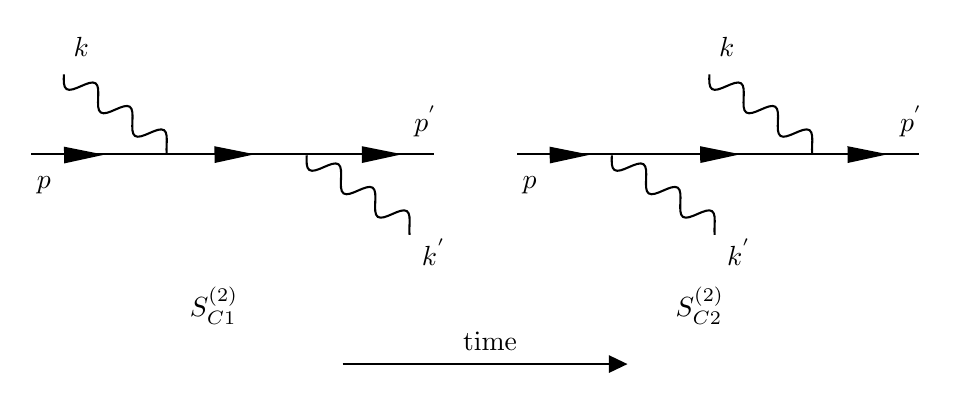
\begin{tikzpicture}[x=0.75pt,y=0.75pt,yscale=-1,xscale=1]
%uncomment if require: \path (0,300); %set diagram left start at 0, and has height of 300

%Straight Lines [id:da9652866719093866] 
\draw    (42,138.93) -- (235.87,138.93) ;
%Shape: Wave [id:dp4726907497917253] 
\draw   (57.65,100.38) .. controls (57.52,103.46) and (57.41,106.39) .. (58.9,107.41) .. controls (60.39,108.44) and (63.08,107.27) .. (65.9,106.03) .. controls (68.72,104.8) and (71.42,103.63) .. (72.91,104.65) .. controls (74.4,105.68) and (74.28,108.61) .. (74.16,111.68) .. controls (74.03,114.76) and (73.91,117.69) .. (75.4,118.71) .. controls (76.9,119.73) and (79.59,118.57) .. (82.41,117.33) .. controls (85.23,116.1) and (87.92,114.93) .. (89.41,115.95) .. controls (90.9,116.98) and (90.79,119.91) .. (90.66,122.98) .. controls (90.53,126.06) and (90.41,128.99) .. (91.9,130.01) .. controls (93.4,131.03) and (96.09,129.86) .. (98.91,128.63) .. controls (101.73,127.4) and (104.42,126.23) .. (105.91,127.25) .. controls (107.41,128.27) and (107.29,131.21) .. (107.16,134.28) .. controls (107.09,135.86) and (107.03,137.39) .. (107.19,138.65) ;
%Shape: Wave [id:dp581219954893428] 
\draw   (174.65,139.38) .. controls (174.52,142.46) and (174.41,145.39) .. (175.9,146.41) .. controls (177.39,147.44) and (180.08,146.27) .. (182.9,145.03) .. controls (185.72,143.8) and (188.42,142.63) .. (189.91,143.65) .. controls (191.4,144.68) and (191.28,147.61) .. (191.16,150.68) .. controls (191.03,153.76) and (190.91,156.69) .. (192.4,157.71) .. controls (193.9,158.73) and (196.59,157.57) .. (199.41,156.33) .. controls (202.23,155.1) and (204.92,153.93) .. (206.41,154.95) .. controls (207.9,155.98) and (207.79,158.91) .. (207.66,161.98) .. controls (207.53,165.06) and (207.41,167.99) .. (208.9,169.01) .. controls (210.4,170.03) and (213.09,168.86) .. (215.91,167.63) .. controls (218.73,166.4) and (221.42,165.23) .. (222.91,166.25) .. controls (224.41,167.27) and (224.29,170.21) .. (224.16,173.28) .. controls (224.09,174.86) and (224.03,176.39) .. (224.19,177.65) ;
%Shape: Triangle [id:dp4781339171474417] 
\draw  [fill={rgb, 255:red, 0; green, 0; blue, 0 }  ,fill opacity=1 ] (74.65,139.08) -- (58.25,142.65) -- (58.19,135.79) -- cycle ;
%Shape: Triangle [id:dp052309184229321404] 
\draw  [fill={rgb, 255:red, 0; green, 0; blue, 0 }  ,fill opacity=1 ] (147.15,138.86) -- (130.75,142.44) -- (130.69,135.57) -- cycle ;
%Shape: Triangle [id:dp3157602553829544] 
\draw  [fill={rgb, 255:red, 0; green, 0; blue, 0 }  ,fill opacity=1 ] (218.15,138.86) -- (201.75,142.44) -- (201.69,135.57) -- cycle ;
%Straight Lines [id:da7163286367875737] 
\draw    (276,138.93) -- (469.87,138.93) ;
%Shape: Wave [id:dp35829325317941596] 
\draw   (368.65,100.38) .. controls (368.52,103.46) and (368.41,106.39) .. (369.9,107.41) .. controls (371.39,108.44) and (374.08,107.27) .. (376.9,106.03) .. controls (379.72,104.8) and (382.42,103.63) .. (383.91,104.65) .. controls (385.4,105.68) and (385.28,108.61) .. (385.16,111.68) .. controls (385.03,114.76) and (384.91,117.69) .. (386.4,118.71) .. controls (387.9,119.73) and (390.59,118.57) .. (393.41,117.33) .. controls (396.23,116.1) and (398.92,114.93) .. (400.41,115.95) .. controls (401.9,116.98) and (401.79,119.91) .. (401.66,122.98) .. controls (401.53,126.06) and (401.41,128.99) .. (402.9,130.01) .. controls (404.4,131.03) and (407.09,129.86) .. (409.91,128.63) .. controls (412.73,127.4) and (415.42,126.23) .. (416.91,127.25) .. controls (418.41,128.27) and (418.29,131.21) .. (418.16,134.28) .. controls (418.09,135.86) and (418.03,137.39) .. (418.19,138.65) ;
%Shape: Wave [id:dp7598034423297523] 
\draw   (321.65,139.38) .. controls (321.52,142.46) and (321.41,145.39) .. (322.9,146.41) .. controls (324.39,147.44) and (327.08,146.27) .. (329.9,145.03) .. controls (332.72,143.8) and (335.42,142.63) .. (336.91,143.65) .. controls (338.4,144.68) and (338.28,147.61) .. (338.16,150.68) .. controls (338.03,153.76) and (337.91,156.69) .. (339.4,157.71) .. controls (340.9,158.73) and (343.59,157.57) .. (346.41,156.33) .. controls (349.23,155.1) and (351.92,153.93) .. (353.41,154.95) .. controls (354.9,155.98) and (354.79,158.91) .. (354.66,161.98) .. controls (354.53,165.06) and (354.41,167.99) .. (355.9,169.01) .. controls (357.4,170.03) and (360.09,168.86) .. (362.91,167.63) .. controls (365.73,166.4) and (368.42,165.23) .. (369.91,166.25) .. controls (371.41,167.27) and (371.29,170.21) .. (371.16,173.28) .. controls (371.09,174.86) and (371.03,176.39) .. (371.19,177.65) ;
%Shape: Triangle [id:dp8027556070300854] 
\draw  [fill={rgb, 255:red, 0; green, 0; blue, 0 }  ,fill opacity=1 ] (308.65,139.08) -- (292.25,142.65) -- (292.19,135.79) -- cycle ;
%Shape: Triangle [id:dp27556888831393467] 
\draw  [fill={rgb, 255:red, 0; green, 0; blue, 0 }  ,fill opacity=1 ] (381.15,138.86) -- (364.75,142.44) -- (364.69,135.57) -- cycle ;
%Shape: Triangle [id:dp8251492979907598] 
\draw  [fill={rgb, 255:red, 0; green, 0; blue, 0 }  ,fill opacity=1 ] (452.15,138.86) -- (435.75,142.44) -- (435.69,135.57) -- cycle ;
%Straight Lines [id:da46165972339858774] 
\draw    (192,239.93) -- (326.17,239.93) ;
\draw [shift={(329.17,239.93)}, rotate = 180] [fill={rgb, 255:red, 0; green, 0; blue, 0 }  ][line width=0.08]  [draw opacity=0] (8.93,-4.29) -- (0,0) -- (8.93,4.29) -- cycle    ;

% Text Node
\draw (48,153.93) node    {$p$};
% Text Node
\draw (232,122.93) node    {$p^{'}$};
% Text Node
\draw (236,185.93) node    {$k^{'}$};
% Text Node
\draw (66,86.93) node    {$k$};
% Text Node
\draw (130,211.93) node    {$S^{( 2)}_{C1}$};
% Text Node
\draw (282,153.93) node    {$p$};
% Text Node
\draw (466,122.93) node    {$p^{'}$};
% Text Node
\draw (383,185.93) node    {$k^{'}$};
% Text Node
\draw (377,86.93) node    {$k$};
% Text Node
\draw (364,211.93) node    {$S^{( 2)}_{C2}$};
% Text Node
\draw (263,228.93) node   [align=left] {time};


\end{tikzpicture}

    \caption{Compton Scattering Can Occur in Two Ways}
    \label{fig:compton-scattering}
\end{figure}
The LH vertex on each side of Fig.(\ref{fig:compton-scattering}) with $x_2$, and the RH with $x_1$, as it would be easier to track the analysis. The interaction could occur in either of the ways we label above as $S_{C 1}^{(2)}$ or $S_{C 2}^{(2)} .$ That is, either i) an electron could absorb a photon (equivalent to an electron and a photon being destroyed and a virtual electron being created at $x_{2}$ ) and later emit a photon(equivalent to the virtual electron being destroyed and both a real electron and a real photon being created at $x_1$); or ii) an electron could emit a photon (equivalent to an electron being destroyed and a real photon along with a virtual electron being created at $x_2$), and later absorbed a photo (equivalent to the virtual electron and a real photon being destroyed while a real electron is create at $x_1$).

\redp{Note that only the $S_{C}^{(2)}$ terms of all the $n=2$ terms will result in destruction of an initial electron and photon ket. }The $S$ matrix transition amplitude for second order Compton scattering is thus (with incoming particles unprimed, outgoing primed)
\begin{equation}
S_{\text {Compton }}=\langle f|S| i\rangle=\left\langle e^-_{\mathbf{p}^{\prime}, s^{\prime}}, \gamma_{\mathbf{k}^{\prime} r^{\prime}}\left|\left(-e^{2}\right) \iint d^{4} x_{1} d^{4} x_{2} N \int\left((\vec{\psi} \linktwoterms{\cancel{A}}{ \psi)_{x_{1}}(\bar{\psi}}{\cancel{A}} \psi)_{x_{2}}\right)\right| e_{\mathbf{p}, s}^{-}, \gamma_{\mathbf{k}, r}\right\rangle
\end{equation}
\begin{equation}
=-e^{2}\left\langle e^-_{\mathbf{p}^{\prime} s^{\prime}}, \gamma_{\mathbf{k}^{\prime}, r^{\prime}}\right| \iint d^{4} x_{1} d^{4} x_{2} N\left\{\left(\bar{\psi}^{+}+\bar{\psi}^{-}\right)_{x_{1}}\left(\cancel{A}^{+}+\cancel{A}^{-}\right)_{x_{1}} \times\right.
\end{equation}
$$
\left.\left(i S_{F}\left(x_{1}-x_{2}\right)\right)\left(\cancel{A}^{+}+\cancel{A}^{-}\right)_{x_{2}}\left(\psi^{+}+\psi^{-}\right)_{x_{2}}\right\}\left|e_{\mathbf{p}, s}^{-}, \gamma_{\mathbf{k}, r}\right\rangle
$$
After the operators raise and lower the ket, only two terms in the equation above remain:
\begin{equation}
\begin{split}
S_{\text {Compton }}&=-e^{2}\left\langle e^-_{\mathbf{p}^{\prime}, s^{\prime}}, \gamma_{\mathbf{k}^{\prime}, r^{\prime}}\right| \iint d^{4} x_{1} d^{4} x_{2} \underbrace{N\left\{\bar{\psi}_{x_{1}}^{-} \cancel{A}_{x_{1}}^{-}\left(i S_{F}\left(x_{1}-x_{2}\right)\right) \cancel{A}_{x_{2}}^{+} \psi_{x_{2}}^{+}\right.}_
{S_{C 1}^{(2)} \text { term } }\\
&+\underbrace{\bar{\psi}_{x_{1}}^{-} \cancel{A}_{x_{1}}^{+}\left(i S_{F}\left(x_{1}-x_{2}\right)\right) \cancel{A}_{x_{2}}^{-} \psi_{x_{2}}^{+}}_{\text {will result in } S_{C_{2}}^{(2)} \text { term }}\}\left|e_{\mathbf{p}, s}^{-}, \gamma_{\mathbf{k}, r}\right\rangle
\end{split}
\end{equation}
\begin{qt}
    The full second order Compton transition amplitude, including both cases of Fig.(\ref{fig:compton-scattering}), is
    \begin{equation}
    \begin{split}
        S_{\text {Compton }}&=\left(\prod_{\mathbf{p}^{''}}^{\text {all fermions }} \sqrt{\frac{m}{V E_{\mathrm{p}^{''}}}}\right)\left(\prod_{\mathbf{p}^{''}}^{\text {all bosons }} \sqrt{\frac{1}{2 V \omega_{\mathbf{k}^{\prime\prime}}}}\right)(2 \pi)^{4}\times\\
        &\delta^{(4)}\left(p^{\prime}+k^{\prime}-p-k\right)\left(\mathcal{M}_{C 1}^{(2)}+\mathcal{M}_{C 2}^{(2)}\right)
    \end{split}
\end{equation}
where
$$
\mathcal{M}_{C 1}^{(2)}=-e^{2} \bar{u}_{s^{\prime}, \alpha}\left(\mathbf{p}^{\prime}\right) \varepsilon_{\mu, r^{\prime}}\left(\mathbf{k}^{\prime}\right) \gamma_{\alpha \beta}^{\mu} i S_{F \beta \delta}(q=p+k) \varepsilon_{\nu, r}(\mathbf{k}) \gamma_{\delta \eta}^{\nu} u_{s, \eta}(\mathbf{p})
$$
$$
\mathcal{M}_{C 2}^{(2)}=-e^{2} \bar{u}_{s^{\prime}, \alpha}\left(\mathbf{p}^{\prime}\right) \varepsilon_{\mu, r}(\mathbf{k}) \gamma_{\alpha \beta}^{\mu} i S_{F \beta \delta}\left(q=p-k^{\prime}\right) \varepsilon_{\nu, r^{\prime}}\left(\mathbf{k}^{\prime}\right) \gamma_{\delta \eta}^{\nu} u_{s, \eta}(\mathbf{p})
$$
\end{qt}
